\documentclass[twoside]{book}

% Packages required by doxygen
\usepackage{fixltx2e}
\usepackage{calc}
\usepackage{doxygen}
\usepackage[export]{adjustbox} % also loads graphicx
\usepackage{graphicx}
\usepackage[utf8]{inputenc}
\usepackage{makeidx}
\usepackage{multicol}
\usepackage{multirow}
\PassOptionsToPackage{warn}{textcomp}
\usepackage{textcomp}
\usepackage[nointegrals]{wasysym}
\usepackage[table]{xcolor}

% Font selection
\usepackage[T1]{fontenc}
\usepackage[scaled=.90]{helvet}
\usepackage{courier}
\usepackage{amssymb}
\usepackage{sectsty}
\renewcommand{\familydefault}{\sfdefault}
\allsectionsfont{%
  \fontseries{bc}\selectfont%
  \color{darkgray}%
}
\renewcommand{\DoxyLabelFont}{%
  \fontseries{bc}\selectfont%
  \color{darkgray}%
}
\newcommand{\+}{\discretionary{\mbox{\scriptsize$\hookleftarrow$}}{}{}}

% Page & text layout
\usepackage{geometry}
\geometry{%
  a4paper,%
  top=2.5cm,%
  bottom=2.5cm,%
  left=2.5cm,%
  right=2.5cm%
}
\tolerance=750
\hfuzz=15pt
\hbadness=750
\setlength{\emergencystretch}{15pt}
\setlength{\parindent}{0cm}
\setlength{\parskip}{3ex plus 2ex minus 2ex}
\makeatletter
\renewcommand{\paragraph}{%
  \@startsection{paragraph}{4}{0ex}{-1.0ex}{1.0ex}{%
    \normalfont\normalsize\bfseries\SS@parafont%
  }%
}
\renewcommand{\subparagraph}{%
  \@startsection{subparagraph}{5}{0ex}{-1.0ex}{1.0ex}{%
    \normalfont\normalsize\bfseries\SS@subparafont%
  }%
}
\makeatother

% Headers & footers
\usepackage{fancyhdr}
\pagestyle{fancyplain}
\fancyhead[LE]{\fancyplain{}{\bfseries\thepage}}
\fancyhead[CE]{\fancyplain{}{}}
\fancyhead[RE]{\fancyplain{}{\bfseries\leftmark}}
\fancyhead[LO]{\fancyplain{}{\bfseries\rightmark}}
\fancyhead[CO]{\fancyplain{}{}}
\fancyhead[RO]{\fancyplain{}{\bfseries\thepage}}
\fancyfoot[LE]{\fancyplain{}{}}
\fancyfoot[CE]{\fancyplain{}{}}
\fancyfoot[RE]{\fancyplain{}{\bfseries\scriptsize Generated by Doxygen }}
\fancyfoot[LO]{\fancyplain{}{\bfseries\scriptsize Generated by Doxygen }}
\fancyfoot[CO]{\fancyplain{}{}}
\fancyfoot[RO]{\fancyplain{}{}}
\renewcommand{\footrulewidth}{0.4pt}
\renewcommand{\chaptermark}[1]{%
  \markboth{#1}{}%
}
\renewcommand{\sectionmark}[1]{%
  \markright{\thesection\ #1}%
}

% Indices & bibliography
\usepackage{natbib}
\usepackage[titles]{tocloft}
\setcounter{tocdepth}{3}
\setcounter{secnumdepth}{5}
\makeindex

% Hyperlinks (required, but should be loaded last)
\usepackage{ifpdf}
\ifpdf
  \usepackage[pdftex,pagebackref=true]{hyperref}
\else
  \usepackage[ps2pdf,pagebackref=true]{hyperref}
\fi
\hypersetup{%
  colorlinks=true,%
  linkcolor=blue,%
  citecolor=blue,%
  unicode%
}

% Custom commands
\newcommand{\clearemptydoublepage}{%
  \newpage{\pagestyle{empty}\cleardoublepage}%
}

\usepackage{caption}
\captionsetup{labelsep=space,justification=centering,font={bf},singlelinecheck=off,skip=4pt,position=top}

%===== C O N T E N T S =====

\begin{document}

% Titlepage & ToC
\hypersetup{pageanchor=false,
             bookmarksnumbered=true,
             pdfencoding=unicode
            }
\pagenumbering{alph}
\begin{titlepage}
\vspace*{7cm}
\begin{center}%
{\Large My Project }\\
\vspace*{1cm}
{\large Generated by Doxygen 1.8.14}\\
\end{center}
\end{titlepage}
\clearemptydoublepage
\pagenumbering{roman}
\tableofcontents
\clearemptydoublepage
\pagenumbering{arabic}
\hypersetup{pageanchor=true}

%--- Begin generated contents ---
\chapter{Hierarchical Index}
\section{Class Hierarchy}
This inheritance list is sorted roughly, but not completely, alphabetically\+:\begin{DoxyCompactList}
\item \contentsline{section}{Boid}{\pageref{class_boid}}{}
\item \contentsline{section}{Flock}{\pageref{class_flock}}{}
\item \contentsline{section}{Obstacle}{\pageref{class_obstacle}}{}
\item Thread\begin{DoxyCompactList}
\item \contentsline{section}{Flock.\+Run\+Parallel}{\pageref{class_flock_1_1_run_parallel}}{}
\end{DoxyCompactList}
\end{DoxyCompactList}

\chapter{Class Index}
\section{Class List}
Here are the classes, structs, unions and interfaces with brief descriptions\+:\begin{DoxyCompactList}
\item\contentsline{section}{\mbox{\hyperlink{class_boid}{Boid}} \\*Class to represent a single unit or boid }{\pageref{class_boid}}{}
\item\contentsline{section}{\mbox{\hyperlink{class_flock}{Flock}} \\*Class to maintain the aggregate behaviour of boids }{\pageref{class_flock}}{}
\item\contentsline{section}{\mbox{\hyperlink{class_obstacle}{Obstacle}} \\*Class to represent the obstacles }{\pageref{class_obstacle}}{}
\item\contentsline{section}{\mbox{\hyperlink{class_flock_1_1_run_parallel}{Flock.\+Run\+Parallel}} \\*Thread class to run the boids in parallel }{\pageref{class_flock_1_1_run_parallel}}{}
\end{DoxyCompactList}

\chapter{Class Documentation}
\hypertarget{class_boid}{}\section{Boid Class Reference}
\label{class_boid}\index{Boid@{Boid}}


Class to represent a single unit or boid.  


\subsection*{Public Member Functions}
\begin{DoxyCompactItemize}
\item 
void \mbox{\hyperlink{class_boid_a3512b360e60eec95f22e1bbaf14d3346}{calc\+\_\+neighbours}} (Array\+List$<$ \mbox{\hyperlink{class_boid}{Boid}} $>$ boids)
\begin{DoxyCompactList}\small\item\em Calculate the neighbours of the boid. \end{DoxyCompactList}\item 
void \mbox{\hyperlink{class_boid_ae286f6aa9f01bed28bc379200c3d7885}{run}} (Array\+List$<$ \mbox{\hyperlink{class_boid}{Boid}} $>$ boids)
\begin{DoxyCompactList}\small\item\em Main function to integrate all the updates of the boid, position, velocity and acceleration. \end{DoxyCompactList}\item 
\mbox{\Hypertarget{class_boid_a86313f583d25e2942a38321a708a2cd7}\label{class_boid_a86313f583d25e2942a38321a708a2cd7}} 
void \mbox{\hyperlink{class_boid_a86313f583d25e2942a38321a708a2cd7}{increment}} ()
\begin{DoxyCompactList}\small\item\em Increment the timer. \end{DoxyCompactList}\item 
void \mbox{\hyperlink{class_boid_a4e57f0bfa16c25001a7b0909185781e4}{apply\+Force}} (P\+Vector force)
\begin{DoxyCompactList}\small\item\em Apply the particular force. \end{DoxyCompactList}\item 
void \mbox{\hyperlink{class_boid_a7a31874a995e7439e894dc0141979ab2}{flock}} (Array\+List$<$ \mbox{\hyperlink{class_boid}{Boid}} $>$ boids)
\begin{DoxyCompactList}\small\item\em Accumulates a new acceleration each time based on three rules. \end{DoxyCompactList}\item 
\mbox{\Hypertarget{class_boid_a688446a89dbcacbd32cfbb49074eee46}\label{class_boid_a688446a89dbcacbd32cfbb49074eee46}} 
void \mbox{\hyperlink{class_boid_a688446a89dbcacbd32cfbb49074eee46}{update}} ()
\begin{DoxyCompactList}\small\item\em Method to update position. \end{DoxyCompactList}\item 
\mbox{\Hypertarget{class_boid_afb58db2cab7b093448fedfdcc09fd276}\label{class_boid_afb58db2cab7b093448fedfdcc09fd276}} 
P\+Vector {\bfseries seek} (P\+Vector target)
\item 
void \mbox{\hyperlink{class_boid_a3dcde93686101c36fbf97a0dd2f2743b}{render}} ()
\begin{DoxyCompactList}\small\item\em Method to render the boid according to the current heading, velocity and position. \end{DoxyCompactList}\item 
void \mbox{\hyperlink{class_boid_a972b44c740e6c93920e66be20ffeed81}{borders}} ()
\begin{DoxyCompactList}\small\item\em Wraparound the boid along corners. \end{DoxyCompactList}\item 
\mbox{\Hypertarget{class_boid_a6d784c3643c0fa5b8865def7f6f63437}\label{class_boid_a6d784c3643c0fa5b8865def7f6f63437}} 
P\+Vector \mbox{\hyperlink{class_boid_a6d784c3643c0fa5b8865def7f6f63437}{separate}} ()
\begin{DoxyCompactList}\small\item\em The rule for the separation of boids. \end{DoxyCompactList}\item 
\mbox{\Hypertarget{class_boid_aecb2dfae64c75103498178e7d1db696b}\label{class_boid_aecb2dfae64c75103498178e7d1db696b}} 
P\+Vector \mbox{\hyperlink{class_boid_aecb2dfae64c75103498178e7d1db696b}{align}} ()
\begin{DoxyCompactList}\small\item\em The rule for the alignmenty of boids. \end{DoxyCompactList}\item 
\mbox{\Hypertarget{class_boid_ae4805e8086160ded6399c44ec6d168fb}\label{class_boid_ae4805e8086160ded6399c44ec6d168fb}} 
P\+Vector \mbox{\hyperlink{class_boid_ae4805e8086160ded6399c44ec6d168fb}{cohesion}} ()
\begin{DoxyCompactList}\small\item\em The rule for the cohesion of boids. \end{DoxyCompactList}\item 
\mbox{\Hypertarget{class_boid_a88de6e18e38e062b6363bfb2741d85f7}\label{class_boid_a88de6e18e38e062b6363bfb2741d85f7}} 
P\+Vector \mbox{\hyperlink{class_boid_a88de6e18e38e062b6363bfb2741d85f7}{avoid\+Obstacles}} ()
\begin{DoxyCompactList}\small\item\em The rule for avoidance of obstacles by the boids. \end{DoxyCompactList}\end{DoxyCompactItemize}
\subsection*{Static Public Member Functions}
\begin{DoxyCompactItemize}
\item 
\mbox{\Hypertarget{class_boid_a350adf423a0d66855334ed5be8a25658}\label{class_boid_a350adf423a0d66855334ed5be8a25658}} 
static void {\bfseries main} ()
\end{DoxyCompactItemize}
\subsection*{Public Attributes}
\begin{DoxyCompactItemize}
\item 
\mbox{\Hypertarget{class_boid_a1c665a132b8231e06e6762fb1c02f369}\label{class_boid_a1c665a132b8231e06e6762fb1c02f369}} 
P\+Vector \mbox{\hyperlink{class_boid_a1c665a132b8231e06e6762fb1c02f369}{position}}
\begin{DoxyCompactList}\small\item\em Vector to show the position of the current boid. \end{DoxyCompactList}\item 
\mbox{\Hypertarget{class_boid_a1229124743705891df66f137e9aa032e}\label{class_boid_a1229124743705891df66f137e9aa032e}} 
P\+Vector \mbox{\hyperlink{class_boid_a1229124743705891df66f137e9aa032e}{velocity}}
\begin{DoxyCompactList}\small\item\em Vector to show the velocity of the current boid. \end{DoxyCompactList}\item 
\mbox{\Hypertarget{class_boid_a945a8f4e1ef0c76118c44d5d735a0d89}\label{class_boid_a945a8f4e1ef0c76118c44d5d735a0d89}} 
P\+Vector \mbox{\hyperlink{class_boid_a945a8f4e1ef0c76118c44d5d735a0d89}{acceleration}}
\begin{DoxyCompactList}\small\item\em Vector to show the acceleration of the current boid. \end{DoxyCompactList}\item 
\mbox{\Hypertarget{class_boid_aab42048b1c1f3efc848eac0f69d1a930}\label{class_boid_aab42048b1c1f3efc848eac0f69d1a930}} 
Array\+List$<$ \mbox{\hyperlink{class_boid}{Boid}} $>$ \mbox{\hyperlink{class_boid_aab42048b1c1f3efc848eac0f69d1a930}{neighbors}}
\begin{DoxyCompactList}\small\item\em Array\+List containing all the neighbours defined by the radius in which they must exist. \end{DoxyCompactList}\item 
\mbox{\Hypertarget{class_boid_ad80d5244136eb1da1723506609ea29a4}\label{class_boid_ad80d5244136eb1da1723506609ea29a4}} 
int \mbox{\hyperlink{class_boid_ad80d5244136eb1da1723506609ea29a4}{decision\+\_\+timer}} = 0
\begin{DoxyCompactList}\small\item\em Time taken by the boid to decide when to change its position. \end{DoxyCompactList}\item 
\mbox{\Hypertarget{class_boid_a3d6ba3f51ea31d95c2d18bc70b884981}\label{class_boid_a3d6ba3f51ea31d95c2d18bc70b884981}} 
float \mbox{\hyperlink{class_boid_a3d6ba3f51ea31d95c2d18bc70b884981}{mass}} = 0.\+058
\begin{DoxyCompactList}\small\item\em Mass of the current boid. \end{DoxyCompactList}\item 
\mbox{\Hypertarget{class_boid_a745696a6bd855bb7ac3464bdc05a2fd5}\label{class_boid_a745696a6bd855bb7ac3464bdc05a2fd5}} 
float \mbox{\hyperlink{class_boid_a745696a6bd855bb7ac3464bdc05a2fd5}{energy}}
\begin{DoxyCompactList}\small\item\em Energy of the current boid. \end{DoxyCompactList}\item 
\mbox{\Hypertarget{class_boid_a38ae17acf614f4f001584e908b6f3333}\label{class_boid_a38ae17acf614f4f001584e908b6f3333}} 
float \mbox{\hyperlink{class_boid_a38ae17acf614f4f001584e908b6f3333}{momentum}}
\begin{DoxyCompactList}\small\item\em Momentum of the current boid. \end{DoxyCompactList}\end{DoxyCompactItemize}


\subsection{Detailed Description}
Class to represent a single unit or boid. 

\subsection{Member Function Documentation}
\mbox{\Hypertarget{class_boid_a4e57f0bfa16c25001a7b0909185781e4}\label{class_boid_a4e57f0bfa16c25001a7b0909185781e4}} 
\index{Boid@{Boid}!apply\+Force@{apply\+Force}}
\index{apply\+Force@{apply\+Force}!Boid@{Boid}}
\subsubsection{\texorpdfstring{apply\+Force()}{applyForce()}}
{\footnotesize\ttfamily void Boid.\+apply\+Force (\begin{DoxyParamCaption}\item[{P\+Vector}]{force }\end{DoxyParamCaption})\hspace{0.3cm}{\ttfamily [inline]}}



Apply the particular force. 

This function simply adds the acceleration passed to it to the total acceleration 
\begin{DoxyParams}{Parameters}
{\em force} & The acceleration which must be added to the total acceleration. \\
\hline
\end{DoxyParams}
\mbox{\Hypertarget{class_boid_a972b44c740e6c93920e66be20ffeed81}\label{class_boid_a972b44c740e6c93920e66be20ffeed81}} 
\index{Boid@{Boid}!borders@{borders}}
\index{borders@{borders}!Boid@{Boid}}
\subsubsection{\texorpdfstring{borders()}{borders()}}
{\footnotesize\ttfamily void Boid.\+borders (\begin{DoxyParamCaption}{ }\end{DoxyParamCaption})\hspace{0.3cm}{\ttfamily [inline]}}



Wraparound the boid along corners. 

Modulo the dimensions of the screen \mbox{\Hypertarget{class_boid_a3512b360e60eec95f22e1bbaf14d3346}\label{class_boid_a3512b360e60eec95f22e1bbaf14d3346}} 
\index{Boid@{Boid}!calc\+\_\+neighbours@{calc\+\_\+neighbours}}
\index{calc\+\_\+neighbours@{calc\+\_\+neighbours}!Boid@{Boid}}
\subsubsection{\texorpdfstring{calc\+\_\+neighbours()}{calc\_neighbours()}}
{\footnotesize\ttfamily void Boid.\+calc\+\_\+neighbours (\begin{DoxyParamCaption}\item[{Array\+List$<$ \mbox{\hyperlink{class_boid}{Boid}} $>$}]{boids }\end{DoxyParamCaption})\hspace{0.3cm}{\ttfamily [inline]}}



Calculate the neighbours of the boid. 

Goes over the boids calculating which of the boids should be included in the neighbours 
\begin{DoxyParams}{Parameters}
{\em boids} & The list containing all boids \\
\hline
\end{DoxyParams}
\mbox{\Hypertarget{class_boid_a7a31874a995e7439e894dc0141979ab2}\label{class_boid_a7a31874a995e7439e894dc0141979ab2}} 
\index{Boid@{Boid}!flock@{flock}}
\index{flock@{flock}!Boid@{Boid}}
\subsubsection{\texorpdfstring{flock()}{flock()}}
{\footnotesize\ttfamily void Boid.\+flock (\begin{DoxyParamCaption}\item[{Array\+List$<$ \mbox{\hyperlink{class_boid}{Boid}} $>$}]{boids }\end{DoxyParamCaption})\hspace{0.3cm}{\ttfamily [inline]}}



Accumulates a new acceleration each time based on three rules. 


\begin{DoxyParams}{Parameters}
{\em boids} & The list containing all boids \\
\hline
\end{DoxyParams}
\mbox{\Hypertarget{class_boid_a3dcde93686101c36fbf97a0dd2f2743b}\label{class_boid_a3dcde93686101c36fbf97a0dd2f2743b}} 
\index{Boid@{Boid}!render@{render}}
\index{render@{render}!Boid@{Boid}}
\subsubsection{\texorpdfstring{render()}{render()}}
{\footnotesize\ttfamily void Boid.\+render (\begin{DoxyParamCaption}{ }\end{DoxyParamCaption})\hspace{0.3cm}{\ttfamily [inline]}}



Method to render the boid according to the current heading, velocity and position. 

Renders the boids accordingly \mbox{\Hypertarget{class_boid_ae286f6aa9f01bed28bc379200c3d7885}\label{class_boid_ae286f6aa9f01bed28bc379200c3d7885}} 
\index{Boid@{Boid}!run@{run}}
\index{run@{run}!Boid@{Boid}}
\subsubsection{\texorpdfstring{run()}{run()}}
{\footnotesize\ttfamily void Boid.\+run (\begin{DoxyParamCaption}\item[{Array\+List$<$ \mbox{\hyperlink{class_boid}{Boid}} $>$}]{boids }\end{DoxyParamCaption})\hspace{0.3cm}{\ttfamily [inline]}}



Main function to integrate all the updates of the boid, position, velocity and acceleration. 


\begin{DoxyParams}{Parameters}
{\em boids} & The list containing all boids \\
\hline
\end{DoxyParams}


The documentation for this class was generated from the following file\+:\begin{DoxyCompactItemize}
\item 
Boid.\+java\end{DoxyCompactItemize}

\hypertarget{class_flock}{}\section{Flock Class Reference}
\label{class_flock}\index{Flock@{Flock}}


Class to maintain the aggregate behaviour of boids.  


\subsection*{Classes}
\begin{DoxyCompactItemize}
\item 
class \mbox{\hyperlink{class_flock_1_1_run_parallel}{Run\+Parallel}}
\begin{DoxyCompactList}\small\item\em Thread class to run the boids in parallel. \end{DoxyCompactList}\end{DoxyCompactItemize}
\subsection*{Public Member Functions}
\begin{DoxyCompactItemize}
\item 
void \mbox{\hyperlink{class_flock_ab97db256aa850e22758daba7874ec611}{run}} ()
\begin{DoxyCompactList}\small\item\em Run the entire flock. \end{DoxyCompactList}\item 
\mbox{\Hypertarget{class_flock_aa290cce57c36e9e7c1c4f2c3695fb896}\label{class_flock_aa290cce57c36e9e7c1c4f2c3695fb896}} 
void {\bfseries add\+Boid} (\mbox{\hyperlink{class_boid}{Boid}} b)
\end{DoxyCompactItemize}
\subsection*{Public Attributes}
\begin{DoxyCompactItemize}
\item 
\mbox{\Hypertarget{class_flock_ab67c86a17efdfb6be0f017f659b7821f}\label{class_flock_ab67c86a17efdfb6be0f017f659b7821f}} 
Array\+List$<$ \mbox{\hyperlink{class_boid}{Boid}} $>$ \mbox{\hyperlink{class_flock_ab67c86a17efdfb6be0f017f659b7821f}{boids}}
\begin{DoxyCompactList}\small\item\em List of boids in the flock. \end{DoxyCompactList}\item 
\mbox{\Hypertarget{class_flock_ad6cf459570d3dee5629b7c67da067a22}\label{class_flock_ad6cf459570d3dee5629b7c67da067a22}} 
float {\bfseries totalenergy}
\item 
\mbox{\Hypertarget{class_flock_a3ef45d17f9335a84a5d025081f416993}\label{class_flock_a3ef45d17f9335a84a5d025081f416993}} 
float \mbox{\hyperlink{class_flock_a3ef45d17f9335a84a5d025081f416993}{totalmomentum}}
\begin{DoxyCompactList}\small\item\em The total momentum of the flock. \end{DoxyCompactList}\item 
\mbox{\Hypertarget{class_flock_af9391becaa97547437cb9b777416a1c0}\label{class_flock_af9391becaa97547437cb9b777416a1c0}} 
int \mbox{\hyperlink{class_flock_af9391becaa97547437cb9b777416a1c0}{notimes}} = 100
\begin{DoxyCompactList}\small\item\em The number of times the display is updated before the speed shown changes. \end{DoxyCompactList}\item 
\mbox{\Hypertarget{class_flock_ac1822e0ef13d9eede3bf25c680f12f40}\label{class_flock_ac1822e0ef13d9eede3bf25c680f12f40}} 
int \mbox{\hyperlink{class_flock_ac1822e0ef13d9eede3bf25c680f12f40}{timer}} = 5
\begin{DoxyCompactList}\small\item\em The timer/clock to look at the changes seen in the flock. \end{DoxyCompactList}\end{DoxyCompactItemize}


\subsection{Detailed Description}
Class to maintain the aggregate behaviour of boids. 

\subsection{Member Function Documentation}
\mbox{\Hypertarget{class_flock_ab97db256aa850e22758daba7874ec611}\label{class_flock_ab97db256aa850e22758daba7874ec611}} 
\index{Flock@{Flock}!run@{run}}
\index{run@{run}!Flock@{Flock}}
\subsubsection{\texorpdfstring{run()}{run()}}
{\footnotesize\ttfamily void Flock.\+run (\begin{DoxyParamCaption}{ }\end{DoxyParamCaption})\hspace{0.3cm}{\ttfamily [inline]}}



Run the entire flock. 

Runs the entire flock code 

The documentation for this class was generated from the following file\+:\begin{DoxyCompactItemize}
\item 
Flock.\+java\end{DoxyCompactItemize}

\hypertarget{class_obstacle}{}\section{Obstacle Class Reference}
\label{class_obstacle}\index{Obstacle@{Obstacle}}


Class to represent the obstacles.  


\subsection*{Public Member Functions}
\begin{DoxyCompactItemize}
\item 
\mbox{\Hypertarget{class_obstacle_adc3b7cfc70a44966762be98d925f57d2}\label{class_obstacle_adc3b7cfc70a44966762be98d925f57d2}} 
void \mbox{\hyperlink{class_obstacle_adc3b7cfc70a44966762be98d925f57d2}{draw}} ()
\begin{DoxyCompactList}\small\item\em Drawing the obstacle at the point specified by the position of the obstacle. \end{DoxyCompactList}\end{DoxyCompactItemize}
\subsection*{Public Attributes}
\begin{DoxyCompactItemize}
\item 
\mbox{\Hypertarget{class_obstacle_a22499e4a7cba1620dac16e0945275bb0}\label{class_obstacle_a22499e4a7cba1620dac16e0945275bb0}} 
P\+Vector \mbox{\hyperlink{class_obstacle_a22499e4a7cba1620dac16e0945275bb0}{position}}
\begin{DoxyCompactList}\small\item\em Represents the position of the obstacle. \end{DoxyCompactList}\end{DoxyCompactItemize}


\subsection{Detailed Description}
Class to represent the obstacles. 

The documentation for this class was generated from the following file\+:\begin{DoxyCompactItemize}
\item 
Obstacle.\+java\end{DoxyCompactItemize}

\hypertarget{class_flock_1_1_run_parallel}{}\section{Flock.\+Run\+Parallel Class Reference}
\label{class_flock_1_1_run_parallel}\index{Flock.\+Run\+Parallel@{Flock.\+Run\+Parallel}}


Thread class to run the boids in parallel.  


Inheritance diagram for Flock.\+Run\+Parallel\+:\begin{figure}[H]
\begin{center}
\leavevmode
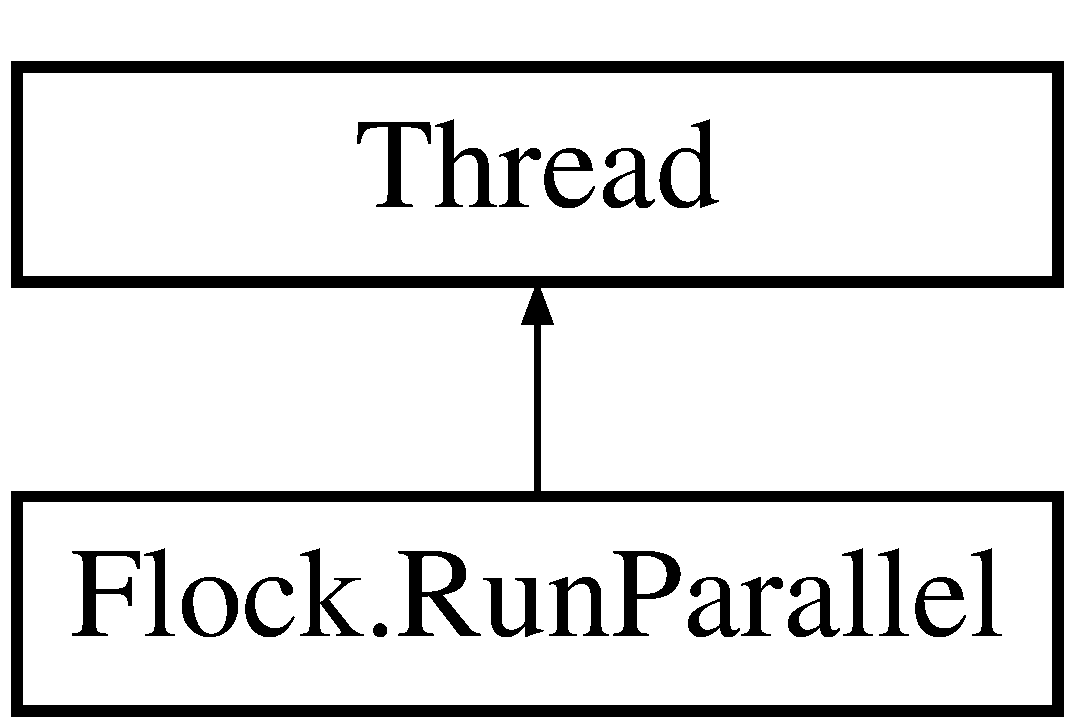
\includegraphics[height=2.000000cm]{class_flock_1_1_run_parallel}
\end{center}
\end{figure}
\subsection*{Public Member Functions}
\begin{DoxyCompactItemize}
\item 
\mbox{\Hypertarget{class_flock_1_1_run_parallel_a122589c3f715c5d43214308a83e9e273}\label{class_flock_1_1_run_parallel_a122589c3f715c5d43214308a83e9e273}} 
{\bfseries Run\+Parallel} (int st, int en, Array\+List$<$ \mbox{\hyperlink{class_boid}{Boid}} $>$ co)
\item 
void \mbox{\hyperlink{class_flock_1_1_run_parallel_a82267b3ef7626f67cb70d5c7bfa65fd1}{run}} ()
\begin{DoxyCompactList}\small\item\em The function to run the thread of the boid array. \end{DoxyCompactList}\end{DoxyCompactItemize}


\subsection{Detailed Description}
Thread class to run the boids in parallel. 

\subsection{Member Function Documentation}
\mbox{\Hypertarget{class_flock_1_1_run_parallel_a82267b3ef7626f67cb70d5c7bfa65fd1}\label{class_flock_1_1_run_parallel_a82267b3ef7626f67cb70d5c7bfa65fd1}} 
\index{Flock\+::\+Run\+Parallel@{Flock\+::\+Run\+Parallel}!run@{run}}
\index{run@{run}!Flock\+::\+Run\+Parallel@{Flock\+::\+Run\+Parallel}}
\subsubsection{\texorpdfstring{run()}{run()}}
{\footnotesize\ttfamily void Flock.\+Run\+Parallel.\+run (\begin{DoxyParamCaption}{ }\end{DoxyParamCaption})\hspace{0.3cm}{\ttfamily [inline]}}



The function to run the thread of the boid array. 

The function is run independent of the other threads and the state of the boids is saved sp that there is no problem due to early updation of the boids in the flock 

The documentation for this class was generated from the following file\+:\begin{DoxyCompactItemize}
\item 
Flock.\+java\end{DoxyCompactItemize}

%--- End generated contents ---

% Index
\backmatter
\newpage
\phantomsection
\clearemptydoublepage
\addcontentsline{toc}{chapter}{Index}
\printindex

\end{document}
